\addtocontents{toc}{\vspace{2em}}
\chapter{Ανάπτυξη λογισμικού με την προσέγγιση συνιστωσών } % Main chapter title

\label{Chapter4} 

\section{Εισαγωγή}
Για την μείωση της πολυπλοκότητας των συστημάτων λογισμικού, οι μηχανικοί λογισμικού έχουν εφεύρει αρκετές τεχνικές που στοχεύουν στην βελτίωση της επαναχρησιμοποίησης και της συντηρησιμότητας του λογισμικού όπως η μοντελοποίηση λογισμικού σε μονάδες (modules) και η αντικειμενοστρέφεια. Στην [33], αναφέρεται ότι το 53\% των συστημάτων λογισμικού δεν πέτυχε να παραδοθεί εντός του χρονοδιαγράμματος και του προϋπολογισμού, καθώς και με την απαιτούμενη λειτουργικότητα και ποιότητα, ενώ το 18\% των έργων εγκαταλείφθηκε πλήρως. Αυτά τα στοιχεία καθιστούν σαφή τη σημασία της ακριβής πρόβλεψης της προσπάθειας που απαιτείται για να αναπτυχθεί ένα νέο σύστημα λογισμικού. 

	Τα τελευταία χρόνια, μία δημοφιλής προσέγγιση ανάπτυξης λογισμικού, η ανάπτυξη λογισμικού βασισμένη σε components (Component Based Software Development, CBSD) έχει αλλάξει σημαντικά την κατάσταση που έχουν να αντιμετωπίσουν οι μηχανικοί λογισμικού. Στην βιομηχανία έχουν αναφερθεί σημαντικά πλεονεκτήματα που δίνει η χρήση της CBSD προσέγγισης ανάπτυξης λογισμικού έναντι του παραδοσιακού τρόπου ανάπτυξης λογισμικού [33]. Μετά την επιτυχία που είχε η Αντικειμενοστραφής προσέγγιση, η CBSD εμφανίζεται ως η επόμενη επανάσταση στον τρόπο ανάπτυξης λογισμικού [34]. Επιπλέον σύμφωνα με την [33] που αφορά τους τρόπους ανάπτυξης λογισμικού που εφαρμόζονται στην βιομηχανία, διαπιστώθηκε ότι περίπου το 53\% από 118 εταιρείες που συμμετείχαν σε έρευνα χρησιμοποιούν την CBSD και η τάση αυτή συνεχώς αυξάνεται. 
	
\section{Η προσέγγιση των συνιστωσών}

\subsection{Γενικές πληροφορίες και βασικές έννοιες}

Η ανάπτυξη λογισμικού με βάση τα components αποτελεί μία προσέγγιση βασισμένη στην επαναχρησιμοποίηση για τον ορισμό, την υλοποίηση και την σύνθεση χαλαρά συνδεδεμένων (loosely coupled) ανεξάρτητων components σε συστήματα λογισμικού. Επιδιώκει να επιφέρει ευρύ φάσμα πλεονεκτημάτων τόσο βραχυπρόθεσμα όσο και μακροπρόθεσμα για το ίδιο το λογισμικό και για οργανισμούς που χορηγούν τέτοιες λύσεις. Το σκεπτικό πίσω από αυτή την προσέγγιση είναι η συναρμολόγηση συστημάτων λογισμικού, χρησιμοποιώντας υπάρχοντα, κατασκευασμένα από τρίτους και δοκιμασμένα components έτσι ώστε να μην είναι απαραίτητη η υλοποίηση όλου του συστήματος από την αρχή. Ο κύκλος ζωής της CBSD μπορεί να χωριστεί σε τέσσερις φάσεις: \textbf{Domain analysis, Component Design and Development, Component Cataloging and Retrieval, Component Selection and Application Assembly} [35]. Κατά την ανάπτυξη ενός προϊόντος λογισμικού χρησιμοποιώντας την CBSD τεχνική, τα διαθέσιμα components συναρμολογούνται ή προσαρμόζονται με τη βοήθεια μίας εφαρμογής ανάπτυξης λογισμικού [34]. Στην εικόνα 4.1 δίνεται μία απεικόνιση της διαδικασίας που ακολουθείται κατά την ανάπτυξη ενός συστήματος λογισμικού χρησιμοποιώντας την CBSD προσέγγιση. 


\begin{figure}[htbp]
	\centering
		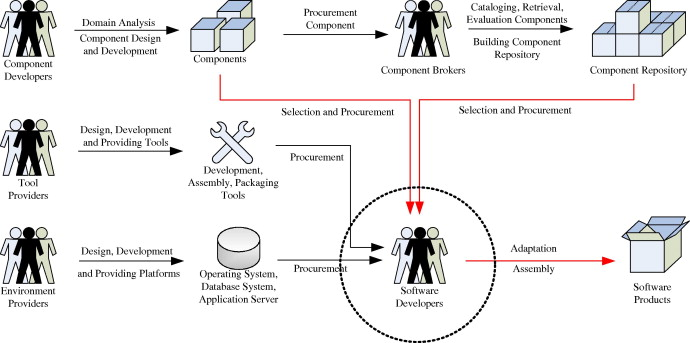
\includegraphics[height=8cm,width=15cm]{Figures/7.jpg}
	\caption{Διάγραμμα ροής της διαδικασίας CBSD \cite{Xie} }	
\end{figure}

\subsection{Οντότητες Λογισμικού}
\subsubsection{Component}
Σύμφωνα με το [36], οι χαρακτηριστικές ιδιότητες ενός component είναι:
\begin{enumerate}
	\item{Αποτελεί μία μονάδα που αναπτύσσεται ανεξάρτητα}
	\item{Μπορεί να αναπτυχθεί και από τρίτους}
	\item{Δεν έχει (εξωτερικά) παρατηρήσιμη κατάσταση}
\end{enumerate}

	Αυτές οι ιδιότητες έχουν πολλές συνέπειες. Για να μπορεί ένα component να αναπτύσσεται ανεξάρτητα, είναι απαραίτητο να διαχωρίζεται από το περιβάλλον στο οποίο θα χρησιμοποιηθεί και από τα άλλα components. Επομένως, ένα component ενθυλακώνει όλα τα χαρακτηριστικά του. Επίσης, καθώς αποτελεί μία μονάδα ανάπτυξης ενός συστήματος δεν θα χρησιμοποιηθεί ποτέ μόνο του. Σε αυτό το πλαίσιο γίνεται σαφές ότι μία ομάδα τρίτων που αναπτύσσει ένα component δεν είναι απαραίτητο να έχει πρόσβαση σε λεπτομέρειες κατασκευής ενός συστήματος καθώς ούτε και σε όλα τα υπόλοιπα components που απαρτίζουν το σύστημα [36]. 
	
	Για να μπορεί ένα component να συνδυαστεί με άλλα components που μπορεί να έχουν σχεδιαστεί και υλοποιηθεί από τρίτους πρέπει να είναι επαρκώς αυτόνομο [36]. Ένα component παρέχει ένα σύνολο υπηρεσιών (services) και τις εκθέτει στο περιβάλλον του μέσω ενός interface που ονομάζεται “provided interface”. Το component επίσης μπορεί να χρειαστεί κάποιες υπηρεσίες από άλλα components ή από το περιβάλλον στο οποίο λειτουργεί προκειμένου να παρέχει με επιτυχία τις δικές του . Αυτές οι απαιτούμενες υπηρεσίες συγκεντρώνονται στο “required interface” του component. Για το λόγο αυτό σε ένα σύστημα που αποτελείται από components κάθε component συναρμολογείται σε συνεργασία με άλλα components ώστε να μπορούν να καλυφθούν οι απαιτήσεις του. Το component ουσιαστικά ορίζει ένα είδος συμβατικής συμφωνίας με την οποία, αν ικανοποιηθούν όλες οι λειτουργικές ανάγκες της (απαιτούμενες υπηρεσίες), καθώς και άλλες πιθανές υποθέσεις για το περιβάλλον ή την πλατφόρμα εκτέλεσης, τότε είναι σε θέση να παρέχει τις λειτουργικές της υπηρεσίες [37]. Με άλλα λόγια, ένα component πρέπει να “κρύβει” την υλοποίηση του από το περιβάλλον του και να αλληλεπιδρά με αυτό μέσω καλά καθορισμένων interfaces [36].

	Τέλος, ένα component δεν πρέπει να έχει οποιαδήποτε εξωτερικά παρατηρήσιμη κατάσταση. Δηλαδή απαιτείται το component να μην διακρίνεται από τα δικά του αντίγραφα. Πιθανές εξαιρέσεις σε αυτό τον κανόνα είναι χαρακτηριστικά που δεν συμβάλουν στην λειτουργικότητα του component, όπως για παράδειγμα οι σειριακοί αριθμοί που χρησιμοποιούνται στην λογιστική. Ο συγκεκριμένος αποκλεισμός της παρατηρήσιμης κατάστασης επιτρέπει τεχνικές χρήσεις της κατάστασης που μπορεί να είναι κρίσιμες για την απόδοση χωρίς να επηρεάζεται η παρατηρήσιμη συμπεριφορά ενός component. Συγκεκριμένα, ένα component μπορεί να χρησιμοποιήσει μια κατάσταση για σκοπούς προσωρινής αποθήκευσης, π.χ. μια μνήμη cache [36].
	
\subsubsection{Interface}

	Τα interfaces αποτελούν σημαντικό στοιχείο των components. Το interface ενός component καθορίζει τις υπηρεσίες που αυτό παρέχει στο περιβάλλον του καθώς και τα σημεία πρόσβασης (access points) του. Κανονικά, ένα component θα απαρτίζεται από πολλά interfaces που θα αντιστοιχούν σε διαφορετικά σημεία πρόσβασης. Κάθε σημείο πρόσβασης μπορεί να παρέχει διαφορετική υπηρεσία, καλύπτοντας διαφορετικές ανάγκες. Ιδιαίτερη έμφαση πρέπει να δοθεί στον συμβατικό χαρακτήρα των προδιαγραφών ενός interface, καθώς το component και τα components που θα το χρησιμοποιήσουν αναπτύσσονται σε αμοιβαία άγνοια, οπότε η σύμβαση (contract) αυτή αποτελεί το κοινό μέσο για την επιτυχή αλληλεπίδραση των components [36]. Η εικόνα 8 δείχνει δύο components με τα interfaces τους.
	
\subsubsection{Container}

	Ο container μπορεί να θεωρηθεί σαν ένας software wrapper γύρω από τα components, ο οποίος είναι υπεύθυνος για την ικανοποίηση των έξω-λειτουργικών απαιτήσεων που τίθενται επί του component. Γενικά, δεν μπορεί να υπάρξει άμεση επικοινωνία μεταξύ των components. Αυτό εν μέρει προκαλείται από τον container μέσα στον οποίο βρίσκεται το component, ο οποίος είναι υπεύθυνος για την απόκτηση και έκθεση των απαιτούμενων και παρεχόμενων interfaces αντίστοιχα. Ο container επίσης, διαμεσολαβεί την πρόσβαση του component σε υπηρεσίες που παρέχονται από την πλατφόρμα εκτέλεσης [37]. Στην εικόνα 4.2 φαίνεται ένα component μαζί με τον container.
	
\subsubsection{Connector}

Ο connector αποτελεί μία οντότητα λογισμικού που είναι υπεύθυνη για την αλληλεπίδραση μεταξύ των components, όπως αυτή ορίζεται από τον container. Ο ρόλος του connector είναι να αποσυνδέσει τα προβλήματα αλληλεπίδρασης από τα προβλήματα λειτουργικότητας. Πρακτικά, αυτό σημαίνει ότι ένα component δεν χειρίζεται άμεσα την αλληλεπίδραση του με τα άλλα components του συστήματος. Έτσι γίνεται εύκολα κατανοητό ότι ο κώδικας ενός component μπορεί να προσδιοριστεί ανεξάρτητα από: (1) τα component στα οποία θα συνδεθεί αργότερα και (2) την μορφή επικοινωνίας που θα χρησιμοποιηθεί. Αυτό είναι απαραίτητο καθώς τα components σχεδιάζονται μεμονωμένα και η σύνδεση τους με άλλα components αποτελεί μεταγενέστερη ανησυχία ή μπορεί να ποικίλει και να είναι σχετική με τα περιβάλλοντα στα οποία θα κληθεί να λειτουργήσει το component [37].


\begin{figure}[htbp]
	\centering
		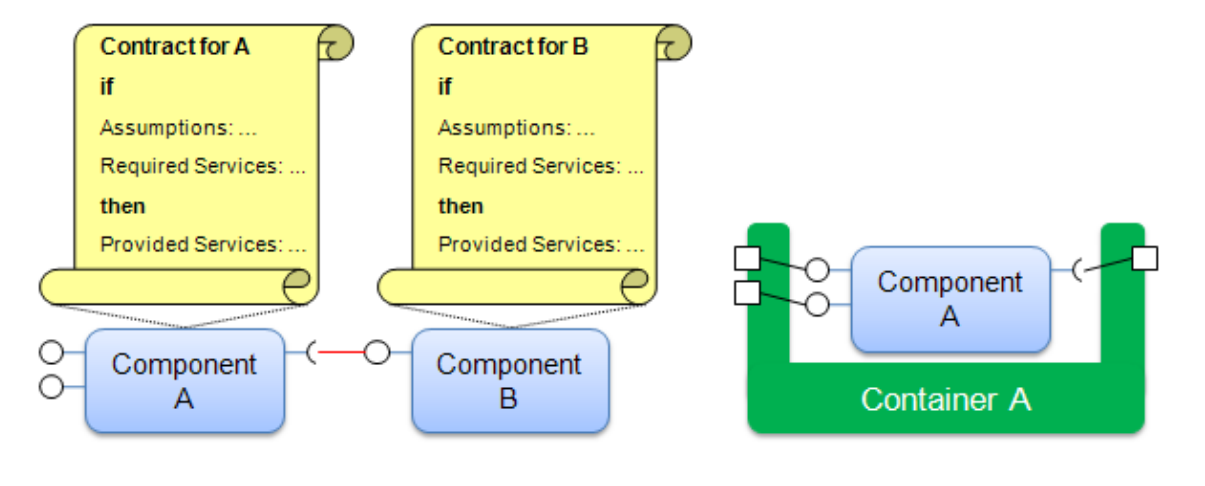
\includegraphics[height=7cm,width=15cm]{Figures/8.png}
	\caption{\textbf{Αριστερά}: Components μαζί με τα interfaces τους. \textbf{Δεξιά}: Ένας container μαζί με το component \cite{Panunzio} }	
\end{figure}

\subsection{Στόχοι της CBSD προσέγγισης}

Υπάρχουν πολλές συζητήσεις και διαφωνίες σχετικά με τι το είναι και τι δεν είναι τα components [38]. Μερικοί συγγραφείς προτιμούν να θεωρούν τα components σαν συνεκτικά πακέτα με χρήσιμη συμπεριφορά, ενώ άλλοι τα αντιμετωπίζουν σαν αναπτυσσόμενες μονάδες λογισμικού που εκτελούνται μέσα σε ένα συγκεκριμένο περιβάλλον [39]. Ανεξάρτητα από αυτές τις διαφορές, η βασική προσέγγιση της CBSD είναι η κατασκευή συστημάτων από σαφώς ορισμένα, ανεξάρτητα μεταξύ τους κομμάτια. Ωστόσο, οι ενδιαφέρουσες πτυχές της CBSD αφορούν τον τρόπο με τον οποίο επιτυγχάνεται αυτή η προσέγγιση, επιτρέποντας την ανάπτυξη των components ως κατάλληλων συνεκτικών μονάδων λειτουργικότητας και τη διευκόλυνση του σχεδιασμού και της συναρμολόγησης συστημάτων από ένα μείγμα νέων και προηγουμένων ανεπτυγμένων components [40]. Ο στόχος της δημιουργίας συστημάτων από καλά καθορισμένα κομμάτια δεν είναι κάτι καινούργιο. 

	Το ενδιαφέρον για την CBSD βασίζεται σε μια μακρά ιστορία εργασίας πάνω σε αρθρωτά συστήματα, δομημένο σχεδιασμό και πιο πρόσφατα σε αντικειμενοστραφή συστήματα [41] - [45]. Αυτά αποσκοπούσαν στην ευκολότερη ανάπτυξη και διατήρηση ευρύτερων συστημάτων χρησιμοποιώντας μια προσέγγιση “divide and conquer”. Η CBSD επεκτείνει αυτές τις ιδέες, δίνοντας έμφαση στο σχεδιασμό λύσεων με κομμάτια λειτουργικότητας που παρέχονται σαν components, προσβάσιμα σε άλλους μόνο μέσω σαφώς ορισμένων interfaces και εστιάζοντας στην ελεγχόμενη συναρμολόγηση των components χρησιμοποιώντας τεχνικές σχεδιασμού βασισμένες σε interfaces [40].


	Το πιο σημαντικό είναι ότι οι έννοιες αυτές υποστηρίζονται από μια σειρά προϊόντων που εφαρμόζουν ανοικτά πρότυπα που προσφέρουν μια υποδομή υπηρεσιών για τη δημιουργία, τη συναρμολόγηση και την εκτέλεση των components. Κατά συνέπεια, η διαδικασία ανάπτυξης εφαρμογών έχει ανασχεδιαστεί έτσι ώστε η κατασκευή λογισμικού να επιτυγχάνεται σε μεγάλο βαθμό μέσω μιας διαδικασίας επιλογής, αξιολόγησης και συναρμολόγησης των components. Τα components αποκτώνται από ένα διαφορετικό σύνολο πηγών και χρησιμοποιούνται μαζί με τοπικά σχεδιασμένο λογισμικό για την κατασκευή μιας πλήρους εφαρμογής [46].
	
\subsection{Γιατί ανάπτυξη λογισμικού με συνιστώσες}
Η ανάπτυξη λογισμικού με βάση τα components, έρχεται να δώσει σημαντικές λύσεις σε πολλές προκλήσεις που αντιμετωπίζει η βιομηχανία καθώς και οι επιχειρήσεις στην εποχή του Διαδικτύου. Αυτές οι προκλήσεις αναφέρονται στην επόμενη λίστα [40]: 

\begin{itemize}
	\item{\textbf{Πολυπλοκότητα}: Σε κάθε περίπλοκη κατάσταση υπάρχουν μερικές βασικές τεχνικές που μπορούν να χρησιμοποιηθούν για την κατανόηση και τη διαχείριση αυτής της πολυπλοκότητας. Αυτές είναι οι τεχνικές αφαίρεσης, αποσύνθεσης και σταδιακής ανάπτυξης. Κάθε λύση ανάπτυξης εφαρμογών πρέπει να παρέχει τρόπους υποστήριξης αυτών των τεχνικών.}
	\item{\textbf{Μείωση του χρόνου παράδοσης}: Η δυνατότητα έγκαιρης παράδοσης λύσεων αποτελεί ουσιαστική πτυχή κάθε έργου ανάπτυξης λογισμικού. Με τον αυξημένο ρυθμό αλλαγής της τεχνολογίας, αυτή η πτυχή γίνεται πιο σημαντική. Αυτή η ανάγκη για μειωμένο χρόνο παράδοσης συστημάτων λογισμικού αναφέρεται συχνά ως εργασίας σε “ρυθμούς Internet”.}
	\item{\textbf{Βελτίωση της συνοχής}: Τα περισσότερα συστήματα λογισμικού μοιράζονται σημαντικά χαρακτηριστικά με άλλα συστήματα που είτε έχουν αναπτυχθεί ήδη, είτε βρίσκονται στην φάση της ανάπτυξης ή δεν έχουν κατασκευαστεί ακόμα. Αν χρησιμοποιηθούν αυτά τα χαρακτηριστικά θα είναι εφικτό να βελτιωθεί η συνοχή και να μειωθεί σημαντικά το κόστος ανάπτυξης νέων συστημάτων λογισμικού. }
	\item{\textbf{Χρήση του καλύτερου στην κατηγορία}: Σε αρκετούς τομείς υπάρχουν ήδη καλά ανεπτυγμένες λύσεις που προσφέρουν ισχυρή λειτουργικότητα και απόδοση. Η αξιοποίηση αυτών των λύσεων ως μέρος μίας μεγαλύτερης προσπάθειας ανάπτυξης ενός συστήματος κρίνεται απαραίτητη. }
	\item{\textbf{Αύξηση της παραγωγικότητας}: Η έλλειψη δεξιοτήτων στον τομέα της ανάπτυξης λογισμικού έχει ως αποτέλεσμα σημαντικές καθυστερήσεις στους χρήστες συστημάτων. Οποιεσδήποτε νέες προσεγγίσεις πρέπει να βελτιώνουν την παραγωγικότητα των εργαζομένων ώστε να μπορούν να παράγουν ποιοτικά αποτελέσματα με ταχύτερους ρυθμούς. }
	\item{\textbf{Βελτίωση της ποιότητας}: Καθώς αυξάνεται το οικονομικό και ανθρώπινο αντίκτυπο μίας αποτυχίας ενός συστήματος λογισμικού, πρέπει να δοθεί ιδιαίτερη προσοχή στην ποιότητα των ανεπτυγμένων συστημάτων. Στόχος πρέπει να είναι η σωστή υποστήριξη της κατασκευής συστημάτων εξ’ αρχής, χωρίς εκτεταμένες και δαπανηρές δοκιμές και επανεγγραφή του κώδικα. }
	\item{\textbf{Αύξηση της ορατότητας στην πρόοδο του έργου}: Η διαχείριση μεγάλων έργων αποτελεί ένα εγχείρημα υψηλού κινδύνου. Για να αποφευχθεί αυτός ο κίνδυνος, πρέπει να είναι δυνατή η μεγαλύτερη ορατότητα καθ’ όλη τη διάρκεια του κύκλου ζωής του λογισμικού. Αυτό απαιτεί μια βαθμιαία προσέγγιση στην ανάπτυξη, την παράδοση και την δοκιμή κομματιών λογισμικού. }
	\item{\textbf{Υποστήριξη παράλληλου και κατανεμημένου τρόπου ανάπτυξης λογισμικού}: Οι κατανεμημένες ομάδες ανάπτυξης λογισμικού απαιτούν προσεγγίσεις που ενθαρρύνουν και επιτρέπουν την παράλληλη ανάπτυξη συστημάτων λογισμικού. Κάτι τέτοιο όμως απαιτεί ιδιαίτερη προσοχή στην διαχείριση της πολυπλοκότητας λόγω της ανάγκης διαίρεσης και επανασυγχρονισμού των αποτελεσμάτων. }
	\item{\textbf{Μείωση του κόστους συντήρησης}: Το μεγαλύτερο μέρους του κόστους ανάπτυξης ενός συστήματος προκύπτει μετά την αρχική ανάπτυξη του συστήματος. Για να μειωθεί το κόστος συντήρησης, πρέπει να είναι δυνατόν να προσδιοριστεί ευκολότερα η ανάγκη για αλλαγή, να είναι εφικτό να προβλεφθεί το αντίκτυπο που θα φέρει οποιαδήποτε προτεινόμενη αλλαγή και να εφαρμοστεί αυτή η αλλαγή στο υπάρχων σύστημα. }
	
\end{itemize}

Η παραπάνω λίστα αποτελεί ένα αποθαρρυντικό σύνολο προκλήσεων για οποιαδήποτε προσέγγιση ανάπτυξης λογισμικού. Ωστόσο, τα components και οι προσεγγίσεις που βασίζονται σε αυτά προσφέρουν την πιο ελπιδοφόρα προσπάθεια αντιμετώπισης των προκλήσεων και προσφέρουν τη βάση μιας νέας σειράς τεχνικών που υποστηρίζουν την επόμενη γενιά λύσεων που προσφέρει το λογισμικό. 

\subsection{Πλεονεκτήματα της CBSD σε σύγκριση με παραδοσιακές τεχνικές ανάπτυξης}

Αρχικά, η φιλοσοφία ανάπτυξης ενός συστήματος λογισμικού αυτών των δύο προσεγγίσεων είναι εντελώς διαφορετική. Η παραδοσιακή ανάπτυξη λογισμικού είναι ίδια με την κατασκευή από το μηδέν. Αντίθετα η CBSD προσέγγιση στηρίζεται περισσότερο στην “buy, don’t build” φιλοσοφία. Δεύτερον, η δομή του λογισμικού που αναπτύσσεται με παραδοσιακές τεχνολογίες χαρακτηρίζεται από υψηλή σύζευξη μεταξύ των επιμέρους τμημάτων του συστήματος, αλλά η CBSD προσπαθεί να κάνει την δομή του λογισμικού να έχει μία χαμηλότερη σύζευξη με σκοπό την βελτίωση της ποιότητας και της συντηρησιμότητας του κώδικα. Η τρίτη σημαντική διαφορά είναι ότι η διαδικασία ανάπτυξης ενός συστήματος λογισμικού χρησιμοποιώντας CBSD είναι εξελικτική και ταυτόχρονη. Αυτό συμβαίνει γιατί ένα σύστημα υλοποιημένο με βάση τα components στην ουσία οικοδομείται και δεν υλοποιείται από την αρχή. Σε αντίθεση με την παραδοσιακή ανάπτυξη λογισμικού, η  CBSD εστιάζει κυρίως σε δραστηριότητες που αφορούν το integration, την αναζήτηση και τον εντοπισμό των υποψήφιων components, την αξιολόγηση και την επιλογή τους βάσει των απαιτήσεων του συστήματος καθώς και των περιορισμών του έργου. Η προσέγγιση CBSD έχει πολλά πλεονεκτήματα, όπως η αποτελεσματική διαχείριση της πολυπλοκότητας, ο μειωμένος χρόνος προς την αγορά, η αυξημένη παραγωγικότητα και ο μεγαλύτερος βαθμός συνοχής και ένα ευρύτερο φάσμα χρηστικότητας. Επιπλέον, τα επαναχρησιμοποιήσιμα στοιχεία καθιστούν δυνατή τη διάσπαση της διαδικασίας ανάπτυξης εφαρμογών σε διαφορετικά μέρη, έτσι ώστε διαφορετικοί άνθρωποι ή εταιρείες να μπορούν να εκτελούν διαφορετικά μέρη της διαδικασίας.


\section{Open Services Gateway initiative (OSGi)}
\subsection{Γενικά}
Από την δεκαετία του ‘70, η οργάνωση του κώδικα σε modules θεωρείται βασική ιδιότητα για την βελτίωση της ευελιξίας, της κατανόησης και της επαναχρησιμοποίησης του [49]. Σε γενικές γραμμές, τα modules αντιστοιχούν σε μονάδες που μπορούν να εκτελέσουν μία διεργασία και μπορούν να υλοποιηθούν ανεξάρτητα, να συγκεντρωθούν και στην συνέχεια να συναρμολογηθούν κατάλληλα ώστε να υλοποιηθεί ένα σύστημα λογισμικού. Για παράδειγμα, οι κλάσεις στην Java ενθυλακώνουν τόσο δεδομένα όσο και υπηρεσίες. Μέσω της τεχνολογίας των πακέτων (packages σε όρους Java), γίνεται ομαδοποίηση και οργάνωση κλάσεων σχετικών μεταξύ τους, με αποτέλεσμα να διευκολύνεται η επαναχρησιμοποίηση. Επιπλέον, τα πακέτα μπορούν να αναπτυχθούν και να διανεμηθούν με την μορφή αρχείων JAR [50]. 

	Ωστόσο το αρθρωτό σύστημα που χρησιμοποιείται στην Java παρουσιάζει τουλάχιστον δύο προβλήματα. Πρώτον, οι μηχανισμοί απόκρυψης πληροφοριών εφαρμόζονται μόνο στο επίπεδο των κλάσεων, αλλά όχι στο επίπεδο των πακέτων και των αρχείων JAR. Για παράδειγμα, δεν είναι δυνατό να περιοριστεί η πρόσβαση σε κλάσεις με ορατότητα public που ορίζονται στα διαθέσιμα πακέτα. Η απουσία τέτοιων κανόνων ελέγχου της ορατότητας μπορεί εύκολα να οδηγήσει σε συστήματα πολύ στενά συνδεδεμένα μεταξύ τους. Από την άλλη πλευρά, το αρθρωτό σύστημα της Java είναι εγγενώς στατικό. Αυτό σημαίνει ότι τα διάφορα modules μπορούν να ενημερωθούν για τυχόν αλλαγές μόνο κατά τον χρόνο ανάπτυξης, γεγονός που απαιτεί διακοπή και επανεκκίνηση του συστήματος [50]. Ένας τέτοιος περιορισμός δημιουργεί τεράστια προβλήματα σε πολλούς τομείς όπως αυτός της βιομηχανίας όπου αναφέρεται και η παρούσα εργασία. 

	Προκειμένου να αντιμετωπιστούν οι περιορισμοί του τυποποιημένου αρθρωτού συστήματος της Java, η πρωτοβουλία  Open Services Gateway (OSGi) πρότεινε το 1999 [48] το  OSGi framework και μοντέλο προγραμματισμού, το οποίο παρέχει ένα δυναμικό αρθρωτό σύστημα με γνώμονα την παροχή υπηρεσιών για την γλώσσα προγραμματισμού Java. Σύμφωνα με τις αρχές του OSGi, τα συστήματα λογισμικού πρέπει να είναι δομημένα γύρω από ανεξάρτητα modules, τα οποία σε όρους OSGi ονομάζονται bundles, που παρέχουν σαφώς καθορισμένες υπηρεσίες. Το OSGi, καθορίζει επίσης και μια υποδομή για τον έλεγχο του κύκλου ζωής των bundles κατά τον χρόνο εκτέλεσης. Αυτή η υποδομή επιτρέπει στους προγραμματιστές να  προσθέτουν, να αφαιρούν και να αναβαθμίζουν bundles από το σύστημα δυναμικά [50]. 
	
\subsection{Η αρχιτεκτονική του OSGi}
Το OSGi παρέχει ένα γενικού σκοπού, ασφαλές και εύκολα διαχειρίσιμο framework για την Java, το οποίο υποστηρίζει την ανάπτυξη επεκτάσιμων εφαρμογών και εφαρμογών που μπορούν να μεταφορτωθούν από το διαδίκτυο, γνωστές και ως bundles. Οι συσκευές που είναι συμβατές με το OSGi μπορούν να λαμβάνουν και να εγκαθιστούν bundles τα οποία θα μπορούν να αφαιρέσουν όταν δεν θα είναι πλέον απαραίτητα. Το framework διαθετει τεχνολογίες που διαχειρίζονται την εγκατάσταση και την ενημέρωση των bundles σε ένα περιβάλλον συμβατό με το OSGi, με δυναμικό και κλιμακωτό τρόπο. Για να επιτευχθεί αυτό, οι εξαρτήσεις (dependencies) μεταξύ των bundles διαχειρίζονται λεπτομερώς από το framework [51].  

	Το OSGi έχει ένα πολυεπίπεδο μοντέλο που απεικονίζεται στην εικόνα 4.3:
	

\begin{figure}[htbp]
	\centering
		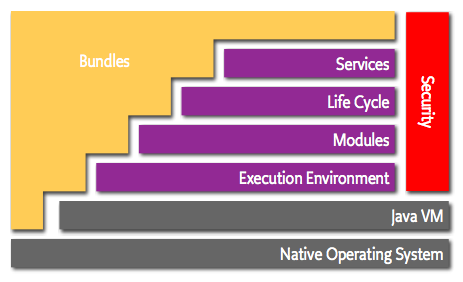
\includegraphics[height=8cm,width=14cm]{Figures/9.png}
	\caption{Τα επίπεδα της αρχιτεκτονικής του OSGi  \cite{OSGi} }	
\end{figure}

\textbf{Bundles}: Τα bundles είναι τα OSGi components που φτιάχνονται από τους προγραμματιστές. Πιο συγκεκριμένα, τα bundles είναι κανονικά .jar αρχεία που περιέχουν αρχεία για τις κλάσεις τους, άλλους πόρους όπως εικόνες, απαιτούμενα API κ. λπ., καθώς και ένα αρχείο manifest το οποίο χρησιμοποιείται για την δήλωση στατικών πληροφοριών σχετικά με το bundle, όπως τα πακέτα που εισάγει και εξάγει. Επιπλέον, κάθε bundle μπορεί να παρέχει υπηρεσίες σε άλλα bundles. Στην αρχιτεκτονική του OSGi, μια υπηρεσία είναι ένα τυπικό αντικείμενο Java που έχει καταχωρηθεί χρησιμοποιώντας έναν ή και περισσότερους τύπους διεπαφών και ιδιοτήτων που χρησιμοποιούνται για τον εντοπισμό της αντίστοιχης υπηρεσίας [50].

	\textbf{Services}: Το επίπεδο των services συνδέει τα bundles με ένα δυναμικό τρόπο προσφέροντας ένα publish-find-bind μοντέλο για τα απλά αντικείμενα Java (POJO). Είναι απαραίτητο γιατί στην Java  είναι δύσκολη η συνεργατική ανάπτυξη κώδικα με κοινή χρήση μόνο των κλάσεων. Η λύση στην Java είναι η χρήση factories που προσφέρουν δυναμική φόρτωση των κλάσεων και των στατικών στοιχείων. Για παράδειγμα αν σε μία εφαρμογή υπάρχει η ανάγκη για την δημιουργία ενός DocumentBuilderFactory θα πρέπει να γίνει κλήση στην στατική μέθοδο του factory DocumentBuilderFactory.newInstance(). Πίσω από αυτή την κλήση όμως, η μέθοδος newInstance() χρησιμοποιεί κάθε τέχνασμα του class loader ώστε να δημιουργήσει ένα νέο instance της κλάσης DocumentBuilderFactory. Αυτό αποτελεί ένα παθητικό μοντέλο. Ο κώδικας της υλοποίησης δεν μπορεί να κάνει τίποτα ώστε να αποδείξει την διαθεσιμότητά του και ο εκάστοτε χρήστης δεν μπορεί να γνωρίζει όλες τις  πιθανές υλοποιήσεις ώστε να διαλέξει την καταλληλότερη. Επιπλέον, είναι ένα στατικό μοντέλο. Μόλις μία υλοποίηση δημιουργήσει ένα νέο instance δεν μπορεί να καταστρέψει το αντικείμενο. Το χειρότερο από όλα είναι ότι αυτό ο μηχανισμός χρησιμοποιείται σε πολλά σημεία και κάθε factory έχει τους δικούς του μοναδικούς μηχανισμούς API και ρύθμισης των παραμέτρων του. Δεν υπάρχει συγκεντρωτική επισκόπηση όλων των υλοποιήσεων του εκάστοτε factory που χρησιμοποιείται. Κάτι τέτοιο δημιουργεί πολλά προβλήματα [48].

	Τη λύση σε όλα αυτά τα προβλήματα δίνει το μητρώο υπηρεσιών που παρέχει το OSGi. Ένα bundle μπορεί να δημιουργήσει ένα αντικείμενο και να το καταχωρήσει στο μητρώο υπηρεσιών κάτω από μία ή περισσότερες διεπαφές. Άλλα bundles μπορούν να μεταβούν στο μητρώο και να βρουν όλα τα αντικείμενα που είναι καταχωρημένα κάτω από μία διεπαφή ή κλάση. Για παράδειγμα, ένα bundle μπορεί να παρέχει μία συγκεκριμένη υλοποίηση του DocumentBuilderIf. Όταν ξεκινάει, δημιουργεί ένα instance του αντικειμένου DocumentBuilderImpl και το καταχωρεί στο μητρώο υπηρεσιών. Ένα bundle που χρειάζεται ένα αντικείμενο DocumentBuilder μπορεί να μεταβεί στο μητρώο και να ζητήσει όλες τις διαθέσιμες υπηρεσίες που υλοποιούν το DocumentBuilderIf. Ακόμα καλύτερα ένα bundle μπορεί να περιμένει μία υπηρεσία να εμφανιστεί και να πάρει μία κλήση πίσω (call back) [48]. 

	Επομένως, ένα bundle μπορεί να καταχωρίσει μία υπηρεσία στο μητρώο, να λάβει μία υπηρεσία που είναι ήδη καταχωρημένη και να περιμένει μία υπηρεσία να εμφανιστεί ή να εξαφανιστεί. Οποιοσδήποτε αριθμός bundles μπορεί να καταχωρίσει την ίδια υπηρεσία και οποιοσδήποτε αριθμός bundles μπορεί να λάβει την ίδια υπηρεσία [48]. Αυτή η λειτουργικότητα εμφανίζεται στην εικόνα 4.4.

	Σύμφωνα με όσα αναφέρθηκαν, είναι εύλογο το ερώτημα πως διαχωρίζονται οι υπηρεσίες αν πολλά bundles έχουν καταχωρήσει την ίδια υπηρεσία. Αρχικά, σε πολλές περιπτώσεις δεν είναι σημαντικό να γίνει διάκριση της υπηρεσίας από ένα συγκεκριμένο bundle. Σε περίπτωση όμως που κάτι τέτοιο κριθεί αναγκαίο το OSGi παρέχει τις ιδιότητες. Κάθε υπηρεσία που καταχωρείται έχει ένα σύνολο από τυπικές και προσαρμοσμένες ιδιότητες. Επιπλέον, υπάρχει μία συγκεκριμένη γλώσσα που μπορεί να φιλτράρει τις υπηρεσίες που παρέχονται και να διαλέξει μόνο αυτές που χρειάζεται το συγκεκριμένο bundle. Οι ιδιότητες μπορούν να χρησιμοποιηθούν για να επιλεχθεί η κατάλληλη υπηρεσία ή να παίξουν και άλλους ρόλους σε επίπεδο εφαρμογής [48].
	
\begin{figure}[htbp]
	\centering
		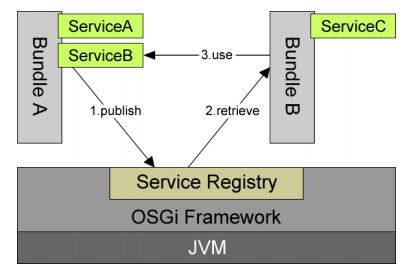
\includegraphics[height=7cm,width=11cm]{Figures/10.png}
	\caption{Το μητρώο υπηρεσίων του OSGi \cite{Tavares} }	
\end{figure}

Οι υπηρεσίες είναι δυναμικές. Αυτό σημαίνει ότι ένα bundle μπορεί να αποφασίσει να  αποσύρει μία υπηρεσία της από το μητρώο, ενώ άλλα bundles εξακολουθούν να χρησιμοποιούν αυτή την υπηρεσία. Τα bundles που χρησιμοποιούν μια τέτοια υπηρεσία πρέπει να διασφαλίζουν ότι δεν χρησιμοποιούν πλέον το αντικείμενο αυτής της υπηρεσίας και να διαγράψουν οποιοδήποτε reference έχουν σε αυτή την υπηρεσία. Αυτό ίσως ακούγεται σαν να επιφέρει σημαντική πολυπλοκότητα αλλά έχουν υλοποιηθεί αρκετές τεχνολογίες οι οποίες λύνουν αυτό το πρόβλημα και επιφέρουν σημαντικά πλεονεκτήματα. Τέτοιες είναι το Service Tracker και τα Declarative Services τα οποία χρησιμοποιήθηκαν στην παρούσα εργασία. Αυτή η δυναμική των υπηρεσιών καθιστά εφικτή την εγκατάσταση και απεγκατάσταση bundles κατά την διάρκεια του run-time και τα υπόλοιπα bundles του συστήματος να μπορούν να προσαρμοστούν. Δηλαδή στην δική μας υλοποίηση μπορούμε να αλλάξουμε το bundle του Valve κατά την διάρκεια που το liqueur θερμαίνεται και το σύστημα να συνεχίζει να δουλεύει κανονικά. 


\textbf{Life-Cycle}: Αποτελεί ένα API για την διαχείριση του κύκλου ζωής των bundles, δηλαδή την εγκατάσταση, την έναρξη, την αναβάθμιση, την διακοπή και την απεγκατάσταση των bundles. Επιπρόσθετα,  παρέχει ένα περιεκτικό API για τα events για να επιτρέπει σε ένα bundle διαχείρισης να ελέγχει τις λειτουργίες του OSGi framework. To επίπεδο Life-Cycle απαιτεί το Module επίπεδο, ενώ το επίπεδο Security δεν είναι απαραίτητο [51]. 

\textbf{Modules}:  Η πλατφόρμα Java προσφέρει περιορισμένη υποστήριξη για τον διαχωρισμό σε πακέτα, την ανάπτυξη και τον έλεγχο εφαρμογών και components που βασίζονται στην γλώσσα Java. Εξαιτίας αυτού, πολλά έργα που βασίζονται σε Java, όπως τα  Jboss και Netbeans, έχουν καταφύγει στην δημιουργία προσαρμοσμένων αντίστοιχων επιπέδων (module layer) με εξειδικευμένους class loaders ώστε να παρέχουν καλύτερη υποστήριξη στην ανάπτυξη, τον διαχωρισμό σε πακέτα και τον έλεγχο εφαρμογών. Το OSGi παρέχει μια γενική και τυποποιημένη λύση για το modularization εφαρμογών.  

	Πιο αναλυτικά, το OSGi ορίζει μία μονάδα (module) το bundle. Ένα bundle αποτελείται από κλάσεις Java και άλλους πόρους, οι οποίοι μαζί μπορούν να παρέχουν λειτουργίες στους τελικούς χρήστες. Τα bundles μπορούν να μοιράζονται πακέτα με άλλα bundles. Στο OSGi τα bundles είναι οι μοναδικές οντότητες για την ανάπτυξη εφαρμογών. Ένα bundle αναπτύσσεται σαν ένα αρχείο .jar. Τα αρχεία .jar συνήθως χρησιμοποιούνται για την αποθήκευση των εφαρμογών και των πόρων τους σε μία τυπική μορφή αρχείου .zip. Ωστόσο, υπάρχει ένας ειδικός τύπος ΜΙΜΕ που προορίζεται για τα OSGi bundles που χρησιμοποιείται για να διακρίνονται τα bundles από κανονικά αρχεία .jar [51]. 

\textbf{Security}: Είναι ένα προαιρετικό επίπεδο που βασίζεται στην αρχιτεκτονική ασφάλειας Java 2. Παρέχει την υποδομή για την ανάπτυξη και την διαχείριση εφαρμογών που πρέπει να εκτελούνται σε ελεγχόμενα και ασφαλή περιβάλλοντα [51]. 

\subsection{Πλεονεκτήματα του OSGi}

Ο βασικός λόγος που το OSGi είναι τόσο επιτυχημένο είναι ότι παρέχει ένα πολύ ώριμο σύστημα για την ανάπτυξη εφαρμογών με την χρήση component, που λειτουργεί σε έναν εκπληκτικό αριθμό περιβάλλοντων. Το OSGi χρησιμοποιείται σε ιδιαίτερα περίπλοκες εφαρμογές όπως περιβάλλοντα ανάπτυξης κώδικα (IDEs), διακομιστές εφαρμογών, gateways καθώς και σε εφαρμογές βιομηχανικού αυτοματισμού. 

	Τα πλεονεκτήματα που παρέχει το OSGi σύμφωνα με το [48] αναφέρονται παρακάτω: 
	
\begin{itemize}
	\item{\textbf{Το OSGi αρχικά δημιουργήθηκε για το ΙοΤ}: Από την αρχή το OSGi είχε σχεδιαστεί με γνώμονα συσκευές με χαμηλή επεξεργαστική ισχύ και μνήμη RAM. Οι συσκευές σήμερα  έχουν μεγαλύτερη επεξεργαστική ισχύ και καλύτερους πόρους. Εξαιτίας αυτού δημιουργήθηκαν εξελιγμένες εφαρμογές και λύσεις καθώς και ακμάζοντα οικοσυστήματα οργανισμών που συνεισφέρουν στην ανάπτυξη λογισμικού. Τέτοια οικοσυστήματα μπορούν να βρεθούν σε ποικίλες αγορές όπως την αγορά των “έξυπνων σπιτιών”, των “έξυπνων” αυτοκινήτων και της Industrie 4.0. Το βιομηχανικό σύστημα παραγωγής λικέρ που χρησιμοποιήθηκε ως μελέτη στην παρούσα διπλωματική εργασία υιοθέτησε σαν βάση το OSGi για την ανάπτυξη του συστήματος παραγωγής myLiquerProduction, το οποίο εκμεταλλεύεται τις τεχνολογίες του ΙοΤ για να επιτρέπει στους τελικούς χρήστες να παράγουν προσαρμοσμένους τύπους λικέρ. Το smartSilo υλοποιήθηκε χρησιμοποιώντας τον hardware προσομοιωτή Silo που είχε αναπτυχθεί σε προηγούμενη διπλωματική εργασία και έναν Controller σε επίπεδο λογισμικού που τρέχει σε Raspberry Pi και αναπτύχθηκε κάτω από το Apache Felix Framework το οποίο αποτελεί μία υλοποίηση ανοιχτού κώδικα του OSGi. }
	\item{\textbf{Μειωμένη πολυπλοκότητα}: Η ανάπτυξη εφαρμογών με το OSGi σημαίνει την ανάπτυξη bundles. Τα bundles κρύβουν τα εσωτερικά στοιχεία τους από τα υπόλοιπα bundles και επικοινωνούν μεταξύ τους μέσω σαφώς καθορισμένων υπηρεσιών. Η απόκρυψη των εσωτερικών στοιχείων προσδίδει μεγαλύτερη ελευθερία στην ανάπτυξη και ευκολία σε οποιαδήποτε αλλαγή που θα επέλθει αργότερα. Κάτι τέτοιο όχι μόνο μειώνει των αριθμό των σφαλμάτων, αλλά κάνει την διαδικασία ανάπτυξης των bundles πιο απλή καθώς κάθε bundle θα υλοποιεί ένα κομμάτι λειτουργικότητας μέσω σαφώς καθορισμένων interfaces. Κάθε component στην συγκεκριμένη εργασία αντιπροσωπεύει αντικείμενα πραγματικού κόσμου του παραδείγματος που υλοποιήθηκε σαν μελέτη, αλλά σε τομέα λογισμικού.}
	\item{\textbf{Επαναχρησιμοποίηση}: Το μοντέλο για τα components που παρέχει το OSGi καθιστά εύκολη τη χρήση πολλών components, που έχουν αναπτυχθεί από τρίτους, σε μία εφαρμογή. Στην υλοποίηση μας χρησιμοποιήθηκαν πολλά τέτοια bundles όπως το Californium for OSGi που είναι μία υλοποίηση του πρωτοκόλλου CoAP σε Java, ο Pax Logger που χρησιμοποιήθηκε σαν logger, η βιβλιοθήκη Pi4J που είναι υπεύθυνη για τον έλεγχο τον General Purpose Inputs Outputs (GPIO) του Raspberry Pi κλπ. }
	\item{\textbf{Δυναμικότητα}: Το μοντέλο του OSGi είναι δυναμικό. Τα διάφορα bundles μπορούν να εγκαθιστώνται, να αναβαθμίζονται, να σταματάνε και να ξεκινούν χωρίς να πρέπει να σταματήσει να λειτουργεί ολόκληρο το σύστημα. Οι περισσότεροι προγραμματιστές δεν θεωρούν ότι κάτι τέτοιο είναι αξιόπιστο και για αυτό το λόγο δεν το χρησιμοποιούν σε πραγματικά περιβάλλοντα. Επιπλέον, στον κόσμο του OSGi οι υπηρεσίες που παρέχει το κάθε bundle μπορεί ανά πάσα στιγμή να μην υπάρχουν. Ωστόσο και ο πραγματικός κόσμος είναι δυναμικός και οι δυναμικές υπηρεσίες που έρχονται και φεύγουν καθιστούν τις δυναμικές υπηρεσίες του OSGi ένα τέλειο μηχανισμό που δίνει λύσει σε πολλά σενάρια πραγματικού κόσμου. Αυτή η δυναμικότητα όμως εξηγείται καλύτερα μέσω ενός παραδείγματος. Στην μελέτη που έγινε στην παρούσα εργασία μία υπηρεσία θα μπορούσε να είναι το άνοιγμα μίας βάνας ενός σιλό. Έστω ότι παρουσιάζεται ένα πρόβλημα και το λογισμικό του controller για τη συγκεκριμένη λειτουργία του συστήματος παρουσιάζει ένα σφάλμα. Τότε μπορεί να αλλαχθεί το bundle που παρέχει την υπηρεσία για το άνοιγμα της βάνας με κάποιο bundle που διορθώνει το πρόβλημα χωρίς να πρέπει να σταματήσει η λειτουργία ολόκληρου του συστήματος. Μόλις το νέο bundle εγκατασταθεί στο περιβάλλον του OSGi και να καταχωρηθεί η νέα υπηρεσία που αυτό παρέχει. Έτσι ο controller βρίσκει τη νέα υπηρεσία και την επόμενη φορά που θα γίνει μία κλήση σε αυτή την μέθοδο θα χρησιμοποιηθεί αυτή. Το συγκεκριμένο παράδειγμα ελέγχθηκε και στην υλοποίηση μας. }
	\item{\textbf{Απλότητα}: Το OSGi είναι εξαιρετικά απλό παρά την διαχείριση των εξαρτήσεων μεταξύ των bundles και της δυναμικότητας που παρέχει. Ο κώδικας σε ένα bundle συμβατό με το OSGi μοιάζει σχεδόν με τον κλασικό κώδικα Java. Ένας συνδυασμός από annotations (Declarative Services) δηλώνουν στο framework πως να χρησιμοποιήσει τον δυναμικό χαρακτήρα του OSGi, καθώς και το ενημερώνουν για τις διάφορες εξαρτήσεις μεταξύ των bundles. Αυτό το πολύ απλό μοντέλο επιτρέπει τη σταδιακή χρήση πιο προηγμένων λειτουργιών. }
\end{itemize}


\subsection{Υλοποιήσεις του OSGi}

Το OSGi είναι ένα τυποποιημένο σύστημα για modules και μία πλατφόρμα υπηρεσιών για την γλώσσα προγραμματισμού Java. Τα πρότυπα του OSGi ορίζονται από την OSGi Alliance και δημοσιεύονται από την ίδια πρωτοβουλία [48]. Αυτή η ενότητα περιέχει μια επισκόπηση των διαθέσιμων υλοποιήσεων του OSGi, τόσο εμπορικές όσο και ανοιχτού κώδικα. Μία γρήγορη επισκόπηση απεικονίζεται στον πίνακα 4.1, που αποτελεί μία τροποποίηση του πίνακα που βρίσκετε στην [53] . 

\begin{table}[h]
\centering
\resizebox{\textwidth}{!}{%
\begin{tabular}{|l|c|c|c|c|}
\hline
\multicolumn{1}{|c|}{} & \textbf{\begin{tabular}[c]{@{}c@{}}Apache Felix\\ (4.4) \\ Open Source\end{tabular}} & \textbf{\begin{tabular}[c]{@{}c@{}}Eclipse Equinox\\ (4.5)\\ Open Source\end{tabular}} & \textbf{\begin{tabular}[c]{@{}c@{}}Knoplerfish\\ (5.1)\\ Open Source\end{tabular}} & \textbf{\begin{tabular}[c]{@{}c@{}}ProSyst\\ (SDK 7.3)\\ Commercial\end{tabular}} \\ \hline
Security (v1.8) & \cellcolor[HTML]{F56B00}1.7 & \cellcolor[HTML]{32CB00}1.8 & \cellcolor[HTML]{F56B00}1.7 & \cellcolor[HTML]{F56B00}1.5 \\ \hline
Core Framework (v6.0) & \cellcolor[HTML]{32CB00}6 & \cellcolor[HTML]{32CB00}6 & \cellcolor[HTML]{32CB00}6 & \cellcolor[HTML]{32CB00}6 \\ \hline
Package Admin Service (v1.2) & \cellcolor[HTML]{32CB00}1.2 & \cellcolor[HTML]{32CB00}1.2 & \cellcolor[HTML]{32CB00}1.2 & \cellcolor[HTML]{32CB00}1.2 \\ \hline
Start Level Service (v1.1) & \cellcolor[HTML]{32CB00}1.1 & \cellcolor[HTML]{32CB00}1.1 & \cellcolor[HTML]{32CB00}1.2 & \cellcolor[HTML]{32CB00}1.2 \\ \hline
Conditional Admin Service (v1.1) & \cellcolor[HTML]{32CB00}1.1 & \cellcolor[HTML]{32CB00}1.1 & \cellcolor[HTML]{32CB00}1.1 & \cellcolor[HTML]{32CB00}1.1 \\ \hline
Permission Admin Service (v1.2) & \cellcolor[HTML]{32CB00}1.2 & \cellcolor[HTML]{32CB00}1.2 & \cellcolor[HTML]{32CB00}1.2 & \cellcolor[HTML]{32CB00}1.2 \\ \hline
URL Handler Service (v1.0) & \cellcolor[HTML]{32CB00}1 & \cellcolor[HTML]{32CB00}1 & \cellcolor[HTML]{32CB00}1 & \cellcolor[HTML]{32CB00}1 \\ \hline
Log	Service (v1.3) & \cellcolor[HTML]{32CB00}1.3 & \cellcolor[HTML]{32CB00}1.3 & \cellcolor[HTML]{32CB00}1.3 & \cellcolor[HTML]{32CB00}1.3 \\ \hline
HTTP Service (v1.2) & \cellcolor[HTML]{32CB00}1.2 & \cellcolor[HTML]{32CB00}1.2 & \cellcolor[HTML]{32CB00}1.2 & \cellcolor[HTML]{32CB00}1.2 \\ \hline
Device Access Service (v1.1) & \cellcolor[HTML]{FE0000}x & \cellcolor[HTML]{32CB00}1.1 & \cellcolor[HTML]{32CB00}1.1 & \cellcolor[HTML]{32CB00}1.1 \\ \hline
Configuration Admin Service (v1.5) & \cellcolor[HTML]{F56B00}1.3 & \cellcolor[HTML]{F56B00}1.3 & \cellcolor[HTML]{32CB00}1.5 & \cellcolor[HTML]{F56B00}1.3 \\ \hline
Meta-type Service (v1.2) & \cellcolor[HTML]{F56B00}1.1 & \cellcolor[HTML]{32CB00}1.2 & \cellcolor[HTML]{32CB00}1.2 & \cellcolor[HTML]{F56B00}1.1 \\ \hline
Preference Service (v1.1) & \cellcolor[HTML]{32CB00}1.1 & \cellcolor[HTML]{32CB00}1.1 & \cellcolor[HTML]{32CB00}1.1 & \cellcolor[HTML]{32CB00}1.1 \\ \hline
User Admin Service (v1.1) & \cellcolor[HTML]{32CB00}1.1 & \cellcolor[HTML]{32CB00}1.1 & \cellcolor[HTML]{32CB00}1.1 & \cellcolor[HTML]{FE0000}x \\ \hline
Wire Admin Service (v1.0) & \cellcolor[HTML]{32CB00}1 & \cellcolor[HTML]{FE0000}x & \cellcolor[HTML]{32CB00}1 & \cellcolor[HTML]{32CB00}1 \\ \hline
IO Connector Service (v1.3) & \cellcolor[HTML]{32CB00}1.3 & \cellcolor[HTML]{FE0000}x & \cellcolor[HTML]{32CB00}1.3 & \cellcolor[HTML]{32CB00}1.3 \\ \hline
Initial Provisioning Service (v1.2) & \cellcolor[HTML]{32CB00}1.2 & \cellcolor[HTML]{FE0000}x & \cellcolor[HTML]{32CB00}1.2 & \cellcolor[HTML]{32CB00}1.2 \\ \hline
UPnP Device Service (v1.2) & \cellcolor[HTML]{F56B00}1.1 & \cellcolor[HTML]{FE0000}x & \cellcolor[HTML]{32CB00}1.2 & \cellcolor[HTML]{F56B00}1.1 \\ \hline
Declarative Service (v1.2) & \cellcolor[HTML]{32CB00}1.2 & \cellcolor[HTML]{32CB00}1.2 & \cellcolor[HTML]{32CB00}1.2 & \cellcolor[HTML]{F56B00}1.1 \\ \hline
Event Admin Service (v1.3) & \cellcolor[HTML]{32CB00}1.3 & \cellcolor[HTML]{32CB00}1.3 & \cellcolor[HTML]{32CB00}1.3 & \cellcolor[HTML]{F56B00}1.2 \\ \hline
Deployment Admin Service (v1.1) & \cellcolor[HTML]{32CB00}1.1 & \cellcolor[HTML]{FE0000}x & \cellcolor[HTML]{32CB00}1.1 & \cellcolor[HTML]{32CB00}1.1 \\ \hline
\end{tabular}%
}
\caption{Διαθέσιμες υλοποιήσεις του OSGi και η έκδοση των modules που υποστηρίζουν}
\label{my-label}
\end{table}

Όπως φαίνεται στον πίνακα 4.1 συγκρίνονται τέσσερις υλοποιήσεις του OSGi, οι τρεις εκ των οποίων είναι ανοιχτού κώδικα. Το \textbf{Apache Felix} αποτελεί μία κοινοτική προσπάθεια για την υλοποίηση του OSGi Framework και άλλων τεχνολογιών που σχετίζονται με το OSGi υπό την άδεια Apache [52]. Αποτελεί την βασική επιλογή των προγραμματιστών που ασχολούνται με το OSGi. Αποτελεί την πιο καθαρή υλοποίηση του OSGi γι’ αυτό και τα modules του που παρέχουν διάφορες υπηρεσίες των προδιαγραφών του OSGi μπορούν να λειτουργήσουν άψογα ακόμα και αν εγκατασταθούν σε κάποια άλλη υλοποίηση. 

	Το \textbf{Knoplerfish} είναι μία υλοποίηση του OSGi που υποστηρίζεται και αναπτύσσεται από την Makewave [54]. Είναι η πιο απλή υλοποίηση του OSGi καθώς έχει σχεδιαστεί για ενσωματωμένα συστήματα και για περιβάλλοντα με περιορισμένους πόρους. Σύμφωνα με την [53], σε μία σύγκριση των παραπάνω υλοποιήσεων αυτή του Knoplerfish αποδείχτηκε η πιο γρήγορη, όταν οι δοκιμές και οι μετρήσεις έγιναν πάνω σε ένα Raspberry Pi. Η συγκεκριμένη υλοποίηση έχει αναπτυχθεί πάνω στο Apache Felix. 

	Το \textbf{Equinox} είναι μία εφαρμογή των προδιαγραφών που ορίζονται από το OSGi, αλλά παρέχει και ένα σύνολο από bundles που υλοποιούν διάφορες προαιρετικές υπηρεσίες του OSGi καθώς και μία υποδομή για τη λειτουργία συστημάτων που βασίζονται στο OSGi. Υποστηρίζεται και αναπτύσσεται από το Eclipse project [55].

	Τέλος, η \textbf{Prosyst} είναι μία από τις πρώτες εταιρείες που συμμετείχαν στην πρωτοβουλία OSGi Alliance και έχει συμβάλλει σημαντικά στην ανάπτυξη των προδιαγραφών του OSGi. Πλέον εστιάζει αποκλειστικά στην ανάπτυξη λογισμικού και λύσεων σχετικών με το OSGi, όπως frameworks, bundles, την υλοποίηση του OSGi που μελετήθηκε σε αυτή την ενότητα. Οι λύσεις που παρέχει χρησιμοποιούνται από συσκευές για το Smart Home, κατασκευαστές αυτοκινήτων, κατασκευαστές κινητών τηλεφώνων κ.α [56]. 

	Στην παρούσα μελέτη, χρησιμοποιήθηκε η υλοποίηση που μας παρέχει το Apache Felix. Αυτό έγινε κυρίως γιατί σκοπός ήταν να δημιουργηθεί ένα περιβάλλον OSGi εξ’ ολοκλήρου από την αρχή ώστε να υπάρχει έλεγχος σε οποιοδήποτε bundle έτρεχε κατά την διάρκεια του run time. Ένα άλλος λόγος που οδηγηθήκαμε σε αυτή την απόφαση ήταν και η υλοποίηση των Core προδιαγραφών του OSGi καθώς την περίοδο που εκπονήθηκε η εργασία οι υπόλοιπες υλοποιήσεις δεν παρείχαν την τελευταία έκδοση αυτών των προδιαγραφών αλλά παρείχαν κάποια προηγούμενη. Αξίζει να σημειωθεί ότι κατά την διάρκεια της εργασίας χρησιμοποιήθηκε και το \textbf{Apache Karaf }το οποίο είναι ένας container βασισμένος σε OSGi χτισμένος πάνω στο Apache Felix. Το Karaf παρέχει πολλές υπηρεσίες χωρίς να χρειάζεται να εγκατασταθούν μία προς μία τις οποίες χρειαστήκαμε στην υλοποίηση μας. Τέτοιες είναι υπηρεσίες όπως οι File Install, Declarative Services, Jetty Server, Felix Webconsole και άλλες που θα αναφερθούν στην συνέχεια. Ωστόσο, στην τελική υλοποίηση χρησιμοποιήσαμε το Apache Felix καθώς ήταν πιο ελαφρύ από το Karaf και μας παρείχε την ίδια λειτουργικότητα.
